% =============================================================================
\section{Introduction}
% =============================================================================

Expert decision-makers do not think equally hard about every choice.
A skilled chess player managing a clock in speed chess plays most moves
quickly, reserving thinking time for the handful of critical positions—the
moves that win or lose the game.
This adaptive allocation of cognitive effort is pervasive in human
reasoning~\citep{griffiths2019doing}, yet it is entirely absent from the
standard reinforcement learning (RL) framework~\citep{travnik2018reactive,
ramstedt2019rtrl}.
In standard RL the environment waits indefinitely for the agent's decision;
computation carries no cost.
Real-time settings break this assumption: the world keeps progressing while
the agent deliberates.
The cost of deliberation is not wall-clock latency in isolation, but
\emph{environmental progression}—ghosts close in, pieces fall under gravity,
clocks deplete—that accumulates while the agent is still deciding.
A perfect action executed one moment too late may be far worse than a timely,
good-enough action.

This real-time structure creates three challenges that standard RL does not
address:
\begin{enumerate}[nosep, leftmargin=*]
  \item \textbf{State-dependence.}
    The right amount of deliberation varies by situation.
    An open board with a distant threat needs little search; a dense board
    with an immediate danger demands deep analysis.
    A fixed thinking budget wastes compute in easy states and underthinks
    critical ones.
  \item \textbf{Intermediate commitment.}
    While the agent deliberates, the environment keeps progressing.
    The agent cannot pause the world—it must commit to some action during
    the delay window, or leave itself exposed.
  \item \textbf{Meta-cost.}
    Deciding \emph{how much} to think could itself require thinking,
    threatening infinite regress.
    The meta-decision must be cheap enough to add negligible real-time cost.
\end{enumerate}

We study this regime using planning-based agents.
Specifically, we use AlphaZero-style models~\citep{silver2018general} that run
Monte Carlo Tree Search (MCTS) at \emph{decision time}: each time the agent
must act, MCTS simulates plausible continuations from the current state,
guided by a neural network's prior and value estimates, and returns a refined
action estimate (see Appendix~\ref{app:az_primer} for a complete description).
The number of MCTS simulations is a clean planning-budget knob: more
simulations yield a better action estimate at the cost of longer inference.
In real-time settings, that inference time is paid as environmental
progression—the cost is in game outcomes, not just latency.
We verify empirically that planning quality and inference latency
co-scale approximately linearly over our simulation ranges
(Figure~\ref{fig:scaling}).
This joint scaling makes the allocation problem tractable: we do not need to
learn \emph{how} to plan, only \emph{when} the marginal quality gain from
additional simulations is worth the additional real-time cost.

This allocation problem is an instance of \textbf{metareasoning}~%
\citep{russell1991right}: the agent must reason not just about which action
to take, but about how much computation that decision deserves.
A long tradition in AI and cognitive science formalizes this as a
\emph{metalevel MDP}—computations are actions at the meta level, each with
an expected value and a cost—and derives a rational rule: invest computation
while its expected gain exceeds its cost~\citep{hay2012selecting,
lieder2017strategy, griffiths2019doing, callaway2018learning}.
Prior metareasoning work has typically treated computation cost as
artificial: a penalty subtracted from reward, or a hard budget externally
imposed.
In our setting, the cost is \emph{physically grounded}: it is the world
advancing while the agent thinks, and the value-of-computation signal emerges
from game outcomes alone, with no reward shaping required.

We address all three challenges with the following design.
We train a standard AlphaZero-style planner and freeze it.
On top, we train a lightweight \textbf{gating policy}~$\pigate(K \mid s_t)$
that reads the current game state and the planner's own value estimate, and
selects a planning budget~$K \in \Kset$.
This generalizes Ramstedt's Real-Time MDP (RTMDP)~\citep{ramstedt2019rtrl},
which fixes the action delay at one timestep, to \emph{variable-delay
real-time RL}, where the agent chooses its own delay at each decision point.
During the $K{-}1$ intermediate steps, the agent executes \textbf{committed
actions}—fast decisions drawn from the frozen planner's own policy logits
(${\sim}2\,$ms each)—that keep the environment moving while MCTS runs in the
background.
On the $K$-th step, the planner's result is applied.
Challenge~(3) dissolves: a single gate forward pass is orders of magnitude
cheaper than one MCTS rollout, so the meta-decision adds negligible real-time
overhead.

We study this setting across two environment classes, each of which makes
deliberation cost real by construction.
In \textbf{committed-action environments} (Pac-Man, Tetris, Snake), the
world evolves during deliberation; the MCTS tree explicitly simulates the
committed-action steps, so search is conducted over the exact future the
agent will experience.
In \textbf{clock environments} (Speed Hex, Speed Go), the remaining time
budget is part of the observation; the value network is trained on
clock-augmented states and therefore prices the cost of thinking directly
into its value estimates.
Both classes share the same gating algorithm and learning procedure.

Our contributions are:
\begin{enumerate}
  \item \textbf{Variable-delay real-time RL.}
    We generalize Ramstedt's fixed-1-step RTMDP to a setting where the agent
    chooses its own delay $K \in \Kset$ at each decision.
    Two physical mechanisms—committed-action progression and explicit
    clocks—instantiate this setting across five environments and make
    deliberation cost real by construction.
  \item \textbf{Adaptive gating policy.}
    We train a lightweight PPO-based gating network on top of a frozen
    AlphaZero planner, formalizing budget selection as a variable-duration
    Semi-Markov Decision Process (SMDP) with per-meta-step
    discount~$\gamma^K$.
  \item \textbf{Empirical validation and deployment transfer.}
    The gating policy consistently outperforms all fixed planning-budget
    baselines in $K \in \Kset$ across all five environments while using less
    average compute, and transfers directly to two-GPU asynchronous
    deployment with no retraining or architectural changes.
\end{enumerate}

The learned gate allocates computation where it matters most.
In Pac-Man, the policy scores 2370 versus the best fixed baseline of
2149 ($+10.3\%$), scaling planning depth with ghost proximity.
In Tetris, it reaches 45.6 versus 27.6 ($+65\%$), learning a bimodal
strategy—react instantly on sparse boards, plan deeply on dense ones.
In Snake, it scores 16.54 versus 14.91 ($+10.9\%$), remaining mostly reactive
($K{=}1$ at 81.6\% of steps) while invoking deeper planning when the board
becomes spatially constrained.
In Speed Hex and Speed Go, the policy remains above parity against
fixed-budget, greedy, midpeak, and random heuristic baselines averaged
across a wide range of clock budgets, shifting toward cheaper options under
time pressure.
In a true two-GPU deployment—environment on one GPU, MCTS on a second—the
trained policy transfers with no modification, confirming that the
committed-action training protocol accurately models the dynamics of
asynchronous execution.

\begin{figure}[t]
  \centering
  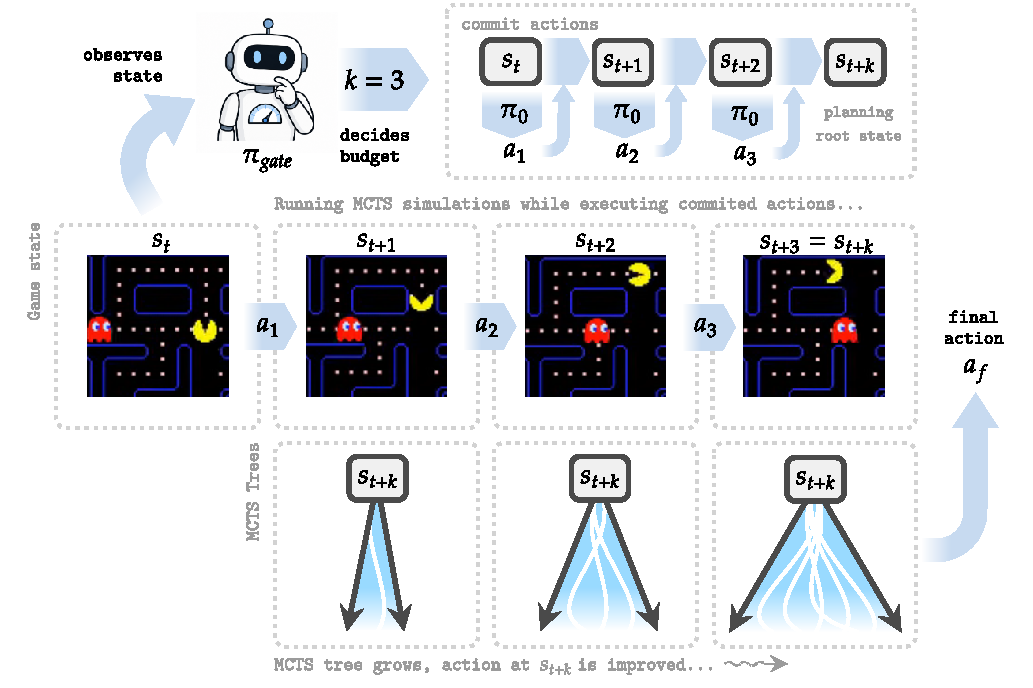
\includegraphics[width=\linewidth]{figures/realtime-rl-gating-diagram.pdf}
  \caption{
    The gating policy chooses whether to react immediately or spend time
    planning.
    Given the current state, a planning budget $K$ is selected, which
    determines how long MCTS runs and, in committed-action environments,
    how many reflex actions are taken.
  }
  \label{fig:realtime-rl-gating-diagram}
\end{figure}

% =============================================================================
\section{Background and Related Work}
% =============================================================================

\paragraph{Metareasoning and the value of computation.}
The central organizing concept of this work is \emph{metareasoning}: the
agent should reason not only about which action to take, but about how much
computation that decision deserves.
\citet{russell1991right} laid the formal groundwork, proposing that rational
agents apply decision theory to the decision of how much to decide—investing
in computation as long as its expected benefit exceeds its cost.
Early work on anytime algorithms~\citep{zilberstein1996using,dean1988analysis}
studied how agents should trade computation against acting now;
real-time heuristic search~\citep{korf1990rta} imposed strict per-move time
limits.
Applied to MCTS, the same idea turns simulation budgeting into a meta-level
control problem~\citep{hay2012selecting,tolpin2012simple,sezener2020static,
lin2015metareasoning}.
The cognitive-science literature sharpens this by modeling bounded
deliberation as a metalevel MDP~\citep{lieder2017strategy,griffiths2019doing,
callaway2018learning}: computations are actions with expected values, and the
agent learns strategies for allocating mental effort.
Prior applications of RL to metareasoning have focused on choosing which
computations to perform~\citep{cope_learning_2023,callaway2018learning};
our contribution is a setting where the cost of computation is physically
grounded in game outcomes rather than externally imposed.

\paragraph{Real-time reinforcement learning.}
Real-time RL reintroduces a cost of deliberation by formalizing environments
that progress during action selection~\citep{travnik2018reactive,
ramstedt2019rtrl}.
Ramstedt's RTMDP augments the state with the action currently in execution,
$\mathbf{x}_t = (s_t, a_t)$, making it equivalent to a constant 1-step
delay MDP~\citep{walsh2009delayed}: the delay is a property of the
framework, not a variable the agent controls.
Extensions handle action and observation delays~\citep{derman2021delayed,
bouteiller2021random,katsikopoulos2003markov} and concurrent
control~\citep{xiao2020thinking}.
Recent work mitigates inference cost through asynchronous and pipelined
architectures~\citep{riemer2025staggered,anokhin2025handling}.
Across all of this work, inference cost is something the architecture
imposes, not something the agent reasons about.
We generalize RTMDP to a variable-delay setting where the agent \emph{chooses}
its delay $K$ at each decision, turning deliberation cost into an explicit
meta-level decision.

\paragraph{Adapting compute per state.}
The closest neighbors to our work \emph{learn} to allocate planning compute.
Metacontrol~\citep{hamrick2017metacontrol} trains a meta-controller to choose
how many imagination steps to run; Thinker and Dynamic
Thinker~\citep{chung2023thinker,wang2024dynamic} let the agent itself decide
when to imagine alternative trajectories; Adaptive
Lookahead~\citep{dalal2022adaptive} learns a state-dependent tree-search
horizon.
\citet{hamrick2021role}'s ablation study provides the strongest empirical
motivation: shallow MuZero trees often suffice, and the marginal value of
additional simulations varies sharply by state.
In parallel, the LLM community has independently advanced the same idea:
adaptive computation time and PonderNet~\citep{graves2016act,banino2021pondernet,
schuster2022calm} learn per-input halting; test-time compute
scaling~\citep{snell2024scaling,deepseek2025r1,muennighoff2025s1} and
RL-trained reasoning-length controllers~\citep{aggarwal2025l1,
muppidi2025predictive,fang2025thinkless,shen2025dast} explicitly learn
per-query thinking budgets; cascaded routing~\citep{kim2023bigl,
chen2023frugalgpt,ong2025routellm} defers easy queries to cheap models.

\paragraph{Our setting.}
We share the thesis that a small learned policy can profitably decide how much
computation to spend per decision—but address a setting none of these works
does.
We gate a \emph{frozen} AlphaZero-style planner, requiring no joint training
between meta-policy and planner.
The cost of deliberation is paid in \emph{environmental progress}, not
artificial reward shaping, so the gating policy learns a value-of-computation
function from outcomes alone.
The committed-action protocol that makes this real-time cost legible during
training also describes the dynamics of true asynchronous execution, so the
trained policy transfers directly to a two-GPU deployment with no retraining
or architectural change.
The options framework~\citep{sutton1999between,bradtke1994reinforcement,
bacon2017optioncritic,harb2018deliberation} and classical MCTS time
management~\citep{baier2016time,huang2010timemanagement,baudis2012pachi}
provide the formal scaffolding for variable-duration meta-decisions and
baselines for our clock environments.
Other axes of ``learning to search''~\citep{guez2018mctsnets,farquhar2018treeqn,
hamrick2020save,racaniere2017i2a} modify the planner's internal behavior rather
than its budget.

% =============================================================================
\section{Real-Time RL Environments}
\label{sec:envs}
% =============================================================================

In a real-time environment the world continues to evolve while the agent
thinks.
That progression can come from adversaries, physics, or explicit clocks:
ghosts close in, gravity pulls pieces downward, the snake body elongates and
constrains future motion, and players' remaining time depletes.
Planning is therefore not merely a computational overhead but a
\emph{meta-reasoning decision}: each simulation spent refining an action is
one more environment step—or fraction of a clock tick—closer to the moment
the action lands.
Figure~\ref{fig:scaling} establishes this concretely: planning quality rises
with simulation count, but so does per-step inference latency, across all GPU
classes tested.

\subsection{Variable-Delay Real-Time RL}
\label{sec:variable_delay}

\textbf{From fixed to variable delay.}
Ramstedt's RTMDP~\citep{ramstedt2019rtrl} formalizes real-time interaction
by augmenting the environment state with the action currently in execution:
$\mathbf{x}_t = (s_t, a_t)$, where $a_t$ was selected one step earlier.
This is mathematically equivalent to a constant 1-step delay
MDP~\citep{walsh2009delayed}: the delay is a fixed property of the framework.
The design is well-suited for lightweight policies whose evaluation fits within
one frame, but it is insufficient for MCTS planning, which can span
$K \in \Kset$ frames ($111$--$444\,$ms at 9\,FPS).
A direct $K$-step extension would require augmenting the state with the $K$
most recent actions, $\mathbf{x}_t = (s_t, a_{t-K+1},\ldots,a_t)$, whose
size grows with $K$; under \emph{variable} $K$, the state dimensionality
would change at each meta-step.

\textbf{Committed actions avoid state augmentation.}
We sidestep this via \emph{committed actions}.
At each meta-step, the gating policy selects $K_t \in \Kset$.
During the $K_t{-}1$ intermediate steps, the agent executes committed actions
$a_\tau = \arg\max_a\,\pi_\theta(a \mid s_\tau)$, computed from the
\emph{current state} $s_\tau$ at each step using a fast forward pass
(${\sim}2\,$ms), not from the stale state $s_0$ where planning began.
On the $K_t$-th step, the MCTS planner's result is applied.
Because each committed action is a deterministic function of the current
state, it does not need to be carried in the state vector to recover the
Markov property.
The MCTS action \emph{is} stale—it was computed at $s_0$ and lands at
$s_{K_t}$—but this staleness is explicitly modeled during training: the
$K_t{-}1$ committed steps actually execute in the environment before the
planner's result is applied, so the policy learns to account for the $K$-step
gap without any state augmentation.

\textbf{SMDP formulation.}
From the meta-policy's perspective, each choice of $K$ defines an
\emph{option}~\citep{sutton1999between}: a $(K,\,\pi_{\mathrm{reflex}})$
pair of length $K$ terminating with the MCTS action.
This yields a Semi-Markov Decision Process (SMDP) with holding time equal to
the chosen $K$ (deterministic in training; slightly stochastic in deployment,
where MCTS latency varies but stays well within the frame budget).
The meta-reward accumulates $\gamma$-discounted environment rewards over all
$K$ steps (Equation~\ref{eq:meta_reward} in Section~\ref{sec:method}), and
the Bellman target carries the per-meta-step discount $\gamma^K$
(Equation~\ref{eq:smdp}).
We adapt Generalized Advantage Estimation~\citep{schulman2015high} to carry
this variable discount through the advantage computation.

\textbf{Cost-awareness by construction.}
Both environment classes make deliberation cost physically real; the mechanism
differs.
In committed-action environments, the MCTS tree explicitly rolls out the
$K{-}1$ committed-action steps internally, so search is conducted over the
same future the agent will actually experience; the cost of a deeper plan is
exactly $K{-}1$ additional steps of world progression before the carefully
chosen action lands.
In clock environments, the value network is trained on observations that
include the remaining time budget, so its estimates already price in the cost
of thinking; a position with little time remaining is worth less than the same
position with ample time.

\subsection{Committed-Action Environments: Pac-Man, Real-Time Tetris, and Snake}

In committed-action environments, acting and planning happen concurrently.
When the gating policy selects budget $K$, it reserves $K$ environment steps
for the planner: the agent takes $K{-}1$ committed actions while MCTS runs in
the background, then applies the planner's result on the $K$-th step
(Figure~\ref{fig:realtime-rl-gating-diagram}).

\paragraph{Equal compute budget.}
All options $K \in \Kset$ are calibrated to the same per-frame simulation
count: at budget $K$, the planner runs $K \times 32$ simulations over $K$
environment steps, giving exactly 32 simulations per game frame on average
(Table~\ref{tab:budget}).
Performance differences therefore reflect \emph{when} compute is invested, not
how much total compute is consumed.

\begin{table}[h]
  \centering
  \caption{Committed-action environments: all $K$ options share 32 MCTS
    simulations per game frame.}
  \label{tab:budget}
  \small
  \begin{tabular}{lcccc}
    \toprule
    & $K{=}1$ & $K{=}2$ & $K{=}3$ & $K{=}4$ \\
    \midrule
    MCTS simulations       & 32 & 64 & 96 & 128 \\
    Committed actions      & 0  & 1  & 2  & 3   \\
    Simulations per frame  & 32 & 32 & 32 & 32  \\
    \bottomrule
  \end{tabular}
\end{table}

\textbf{Jumanji environments.}
We study three committed-action environments derived from
Jumanji~\citep{bonnet2024jumanji}: Pac-Man, Snake, and a real-time variant of
Tetris.
In Pac-Man, ghosts and the player continue moving while search runs.
In Tetris, we modify the Jumanji environment so that gravity advances the
falling piece in real time (Appendix~\ref{app:envs_tetris}).
In Snake, each committed step moves the snake forward, changing its body
occupancy and the spatial constraints on future actions.
The common structure is that a deeper plan arrives later, after the world has
already changed.
In all three cases, the MCTS tree accounts for the committed-action delay
explicitly: its simulation function rolls out the $K{-}1$ committed steps
internally using the planner's argmax policy, making the search model match
the deployment-time behavior.

\subsection{Clock Environments: Speed Hex and Speed Go}

In clock environments, the agent's remaining time is part of the observation
and the network is trained to be budget-aware.
MCTS simulations use board-only dynamics (no clock deduction during search),
but because the network has always observed the clock state during training,
its value estimates already price in the cost of thinking: a position with
little time remaining is worth less than the same position with ample time.
When the agent chooses budget $K$, the corresponding time cost is deducted
from the clock after the move is played.
Committed actions during the planning phase are no-ops: since the board does
not evolve while a player deliberates, the only resource being consumed is
clock.
The SMDP discount $\gamma^K$ therefore captures both standard time-discounting
and the implicit opportunity cost of the clock ticks spent planning.

We study this setting in Speed Hex ($11{\times}11$) and Speed Go ($9{\times}9$),
both built on the pgx game library.
In both games the key choice is not only \emph{which} move to play but
\emph{how much} of the remaining clock to spend before playing it.
Simulation options are calibrated so that each option represents a
meaningfully distinct quality--latency tradeoff
(Appendix~\ref{app:sim_calibration}): $\{2,8,32,128\}$ simulations for Speed
Hex and $\{16,32,64,96\}$ for Speed Go.
Because the policy is trained across many clock settings, its strategy
generalizes across budgets rather than being tuned at each level
separately—the gating policy adapts its allocation to the remaining time
rather than memorizing a fixed strategy.
